% whatif-flow.tex -- the path of one what-if (E8 and E9), from a keystroke to the charts
% COS30049 Assignment 3, Bitcoin Address Activity Explorer. Drawn from the code on main (21 Nov 2026).
% Compiles on its own:  pdflatex whatif-flow.tex   (one cropped page; needs only tikz and lmodern).
% It does not use the standalone class, which a small TeX installation may lack; the last lines of
% this file crop the page to the picture instead. To place it in the report: 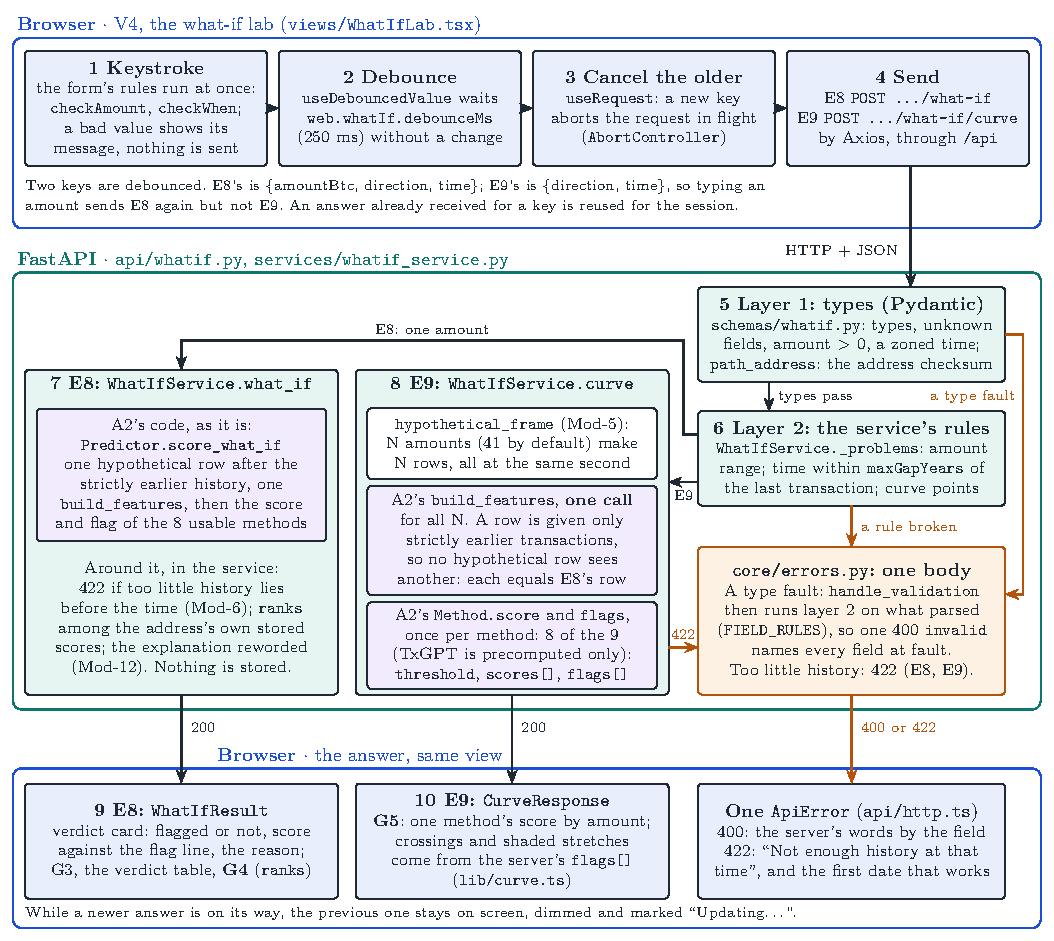
\includegraphics{whatif-flow.pdf}.
% The boxes, words and arrows are the same as in whatif-flow.svg; README.md lists the source file behind each.

\documentclass{article}
\usepackage[T1]{fontenc}
\usepackage{lmodern}
\usepackage{tikz}
\usetikzlibrary{arrows.meta, backgrounds}
% The plan's colours (docs/plan/main.tex).
\definecolor{ink}{HTML}{1F2933}
\definecolor{accent}{HTML}{1D4ED8}
\definecolor{accentsoft}{HTML}{E8EEFC}
\definecolor{teal}{HTML}{0F766E}
\definecolor{tealsoft}{HTML}{E6F4F2}
\definecolor{violet}{HTML}{6D28D9}
\definecolor{violetsoft}{HTML}{F1EBFD}
\definecolor{grey}{HTML}{6B7280}
\definecolor{greysoft}{HTML}{F3F4F6}
\definecolor{warn}{HTML}{B45309}
\definecolor{warnsoft}{HTML}{FDF1E3}
\pagestyle{empty}
\newsavebox{\figbox}
\newlength{\figborder}\setlength{\figborder}{6pt}
\begin{document}
\begin{lrbox}{\figbox}%
\frenchspacing
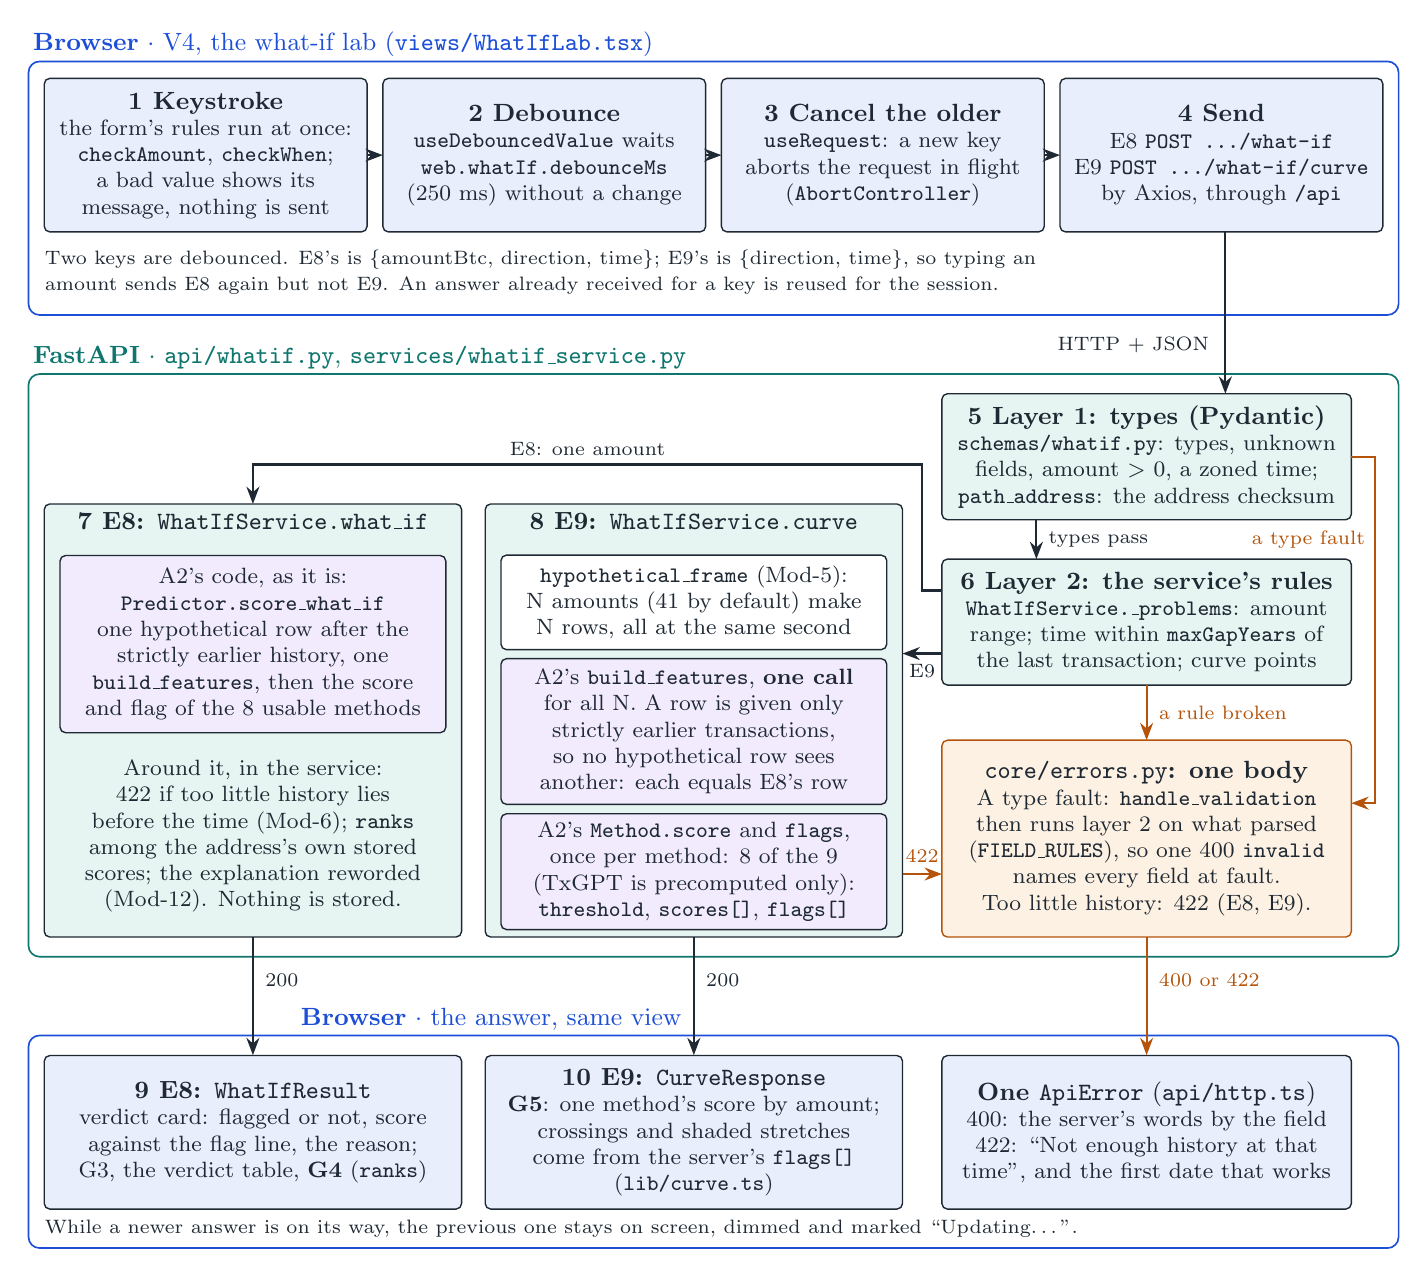
\begin{tikzpicture}[x=1cm, y=1cm, font=\footnotesize, text=ink,
  box/.style={draw=ink, rounded corners=2pt, align=center, inner sep=3pt, line width=0.5pt},
  fe/.style={box, fill=accentsoft}, be/.style={box, fill=tealsoft}, ml/.style={box, fill=violetsoft},
  st/.style={box, fill=greysoft}, er/.style={box, fill=warnsoft, draw=warn}, plain/.style={box, fill=white},
  txt/.style={align=center, inner sep=0pt},
  grp/.style={rounded corners=4pt, line width=0.6pt},
  arr/.style={-{Stealth[length=2.2mm]}, thick, draw=ink},
  darr/.style={{Stealth[length=2.2mm]}-{Stealth[length=2.2mm]}, thick, draw=ink},
  opt/.style={arr, dashed},
  err/.style={arr, draw=warn},
  bare/.style={thick, draw=ink}]
  % ---- groups (frames behind everything)
  \draw[grp, draw=accent] (-0.20,-3.00) rectangle (17.20,0.22);
  \node[anchor=south west, inner sep=1.5pt, text=accent, font=\small] at (-0.20,0.22) {\textbf{Browser} $\cdot$ V4, the what-if lab (\texttt{views/WhatIfLab.tsx})};
  \draw[grp, draw=teal] (-0.20,-11.15) rectangle (17.20,-3.75);
  \node[anchor=south west, inner sep=1.5pt, text=teal, font=\small] at (-0.20,-3.75) {\textbf{FastAPI} $\cdot$ \texttt{api/whatif.py}, \texttt{services/whatif\_service.py}};
  \draw[grp, draw=accent] (-0.20,-14.85) rectangle (17.20,-12.15);
  \node[anchor=south west, inner sep=1.5pt, text=accent, font=\small] at (3.20,-12.15) {\textbf{Browser} $\cdot$ the answer, same view};
  % ---- boxes
  \node[fe, minimum width=4.10cm, minimum height=1.95cm] (k1) at (2.05,-0.97) {{\small \textbf{1  Keystroke}}\\ the form's rules run at once:\\ \texttt{checkAmount}, \texttt{checkWhen};\\ a bad value shows its\\ message, nothing is sent};
  \node[fe, minimum width=4.10cm, minimum height=1.95cm] (k2) at (6.35,-0.97) {{\small \textbf{2  Debounce}}\\ \texttt{useDebouncedValue} waits\\ \texttt{web.whatIf.debounceMs}\\ (250 ms) without a change};
  \node[fe, minimum width=4.10cm, minimum height=1.95cm] (k3) at (10.65,-0.97) {{\small \textbf{3  Cancel the older}}\\ \texttt{useRequest}: a new key\\ aborts the request in flight\\ (\texttt{AbortController})};
  \node[fe, minimum width=4.10cm, minimum height=1.95cm] (k4) at (14.95,-0.97) {{\small \textbf{4  Send}}\\ E8 \texttt{POST .../what-{}if}\\ E9 \texttt{POST .../what-{}if/curve}\\ by Axios, through \texttt{/api}};
  \node[be, minimum width=5.20cm, minimum height=1.60cm] (v5) at (14.00,-4.80) {{\small \textbf{5  Layer 1: types (Pydantic)}}\\ \texttt{schemas/whatif.py}: types, unknown\\ fields, amount \textgreater{} 0, a zoned time;\\ \texttt{path\_address}: the address checksum};
  \node[be, minimum width=5.20cm, minimum height=1.60cm] (v6) at (14.00,-6.90) {{\small \textbf{6  Layer 2: the service's rules}}\\ \texttt{WhatIfService.\_problems}: amount\\ range; time within \texttt{maxGapYears} of\\ the last transaction; curve points};
  \node[er, minimum width=5.20cm, minimum height=2.50cm] (verr) at (14.00,-9.65) {{\small \textbf{\texttt{core/errors.py}}\textbf{: one body}}\\ A type fault: \texttt{handle\_validation}\\ then runs layer 2 on what parsed\\ (\texttt{FIELD\_RULES}), so one 400 \texttt{invalid}\\ names every field at fault.\\ Too little history: 422 (E8, E9).};
  \node[be, minimum width=5.30cm, minimum height=5.50cm] (e8) at (2.65,-8.15) {};
  \node[txt, align=center, anchor=north] at (2.65,-5.50) {{\small \textbf{7  E8: }\textbf{\texttt{WhatIfService.what\_if}}}};
  \node[ml, minimum width=4.90cm, minimum height=2.25cm] (e8a) at (2.65,-7.18) {A2's code, as it is:\\ \textbf{\texttt{Predictor.score\_what\_if}}\\ one hypothetical row after the\\ strictly earlier history, one\\ \texttt{build\_features}, then the score\\ and flag of the 8 usable methods};
  \node[txt] (e8b) at (2.65,-9.62) {Around it, in the service:\\ 422 if too little history lies\\ before the time (Mod-6); \texttt{ranks}\\ among the address's own stored\\ scores; the explanation reworded\\ (Mod-12). Nothing is stored.};
  \node[be, minimum width=5.30cm, minimum height=5.50cm] (e9) at (8.25,-8.15) {};
  \node[txt, align=center, anchor=north] at (8.25,-5.50) {{\small \textbf{8  E9: }\textbf{\texttt{WhatIfService.curve}}}};
  \node[plain, minimum width=4.90cm, minimum height=1.20cm] (e9a) at (8.25,-6.65) {\texttt{hypothetical\_frame} (Mod-5):\\ N amounts (41 by default) make\\ N rows, all at the same second};
  \node[ml, minimum width=4.90cm, minimum height=1.85cm] (e9b) at (8.25,-8.29) {A2's \texttt{build\_features}, \textbf{one call}\\ for all N. A row is given only\\ strictly earlier transactions,\\ so no hypothetical row sees\\ another: each equals E8's row};
  \node[ml, minimum width=4.90cm, minimum height=1.46cm] (e9c) at (8.25,-10.07) {A2's \texttt{Method.score} and \texttt{flags},\\ once per method: 8 of the 9\\ (TxGPT is precomputed only):\\ \texttt{threshold}, \texttt{scores[]}, \texttt{flags[]}};
  \node[fe, minimum width=5.30cm, minimum height=1.95cm] (r8) at (2.65,-13.38) {{\small \textbf{9  E8: }\textbf{\texttt{WhatIfResult}}}\\ verdict card: flagged or not, score\\ against the flag line, the reason;\\ G3, the verdict table, \textbf{G4} (\texttt{ranks})};
  \node[fe, minimum width=5.30cm, minimum height=1.95cm] (r9) at (8.25,-13.38) {{\small \textbf{10  E9: }\textbf{\texttt{CurveResponse}}}\\ \textbf{G5}: one method's score by amount;\\ crossings and shaded stretches\\ come from the server's \texttt{flags[]}\\ (\texttt{lib/curve.ts})};
  \node[fe, minimum width=5.20cm, minimum height=1.95cm] (rerr) at (14.00,-13.38) {{\small \textbf{One }\textbf{\texttt{ApiError}} (\texttt{api/http.ts})}\\ 400: the server's words by the field\\ 422: ``Not enough history at that\\ time'', and the first date that works};
  % ---- arrows
  \draw[arr] (4.10,-0.97) -- (4.30,-0.97);
  \draw[arr] (8.40,-0.97) -- (8.60,-0.97);
  \draw[arr] (12.70,-0.97) -- (12.90,-0.97);
  % 4 -> 5
  \draw[arr] (15.00,-1.95) -- (15.00,-4.00);
  % 5 -> 6
  \draw[arr] (12.60,-5.60) -- (12.60,-6.10);
  % 5 -> errors (type fault)
  \draw[err] (16.60,-4.80) -- (16.90,-4.80) -- (16.90,-9.20) -- (16.60,-9.20);
  % 6 -> errors (rule broken: InvalidRequest)
  \draw[err] (14.00,-7.70) -- (14.00,-8.40);
  % 6 -> 7 (E8)
  \draw[arr] (11.40,-6.50) -- (11.15,-6.50) -- (11.15,-4.90) -- (2.65,-4.90) -- (2.65,-5.40);
  % 6 -> 8 (E9)
  \draw[arr] (11.40,-7.30) -- (10.90,-7.30);
  % E8/E9 -> errors (422)
  \draw[err] (10.90,-10.10) -- (11.40,-10.10);
  % E8 -> verdict card, G3, G4
  \draw[arr] (2.65,-10.90) -- (2.65,-12.40);
  % E9 -> G5
  \draw[arr] (8.25,-10.90) -- (8.25,-12.40);
  % error body -> ApiError
  \draw[err] (14.00,-10.90) -- (14.00,-12.40);
  % ---- labels
  \node[txt, anchor=west, font=\scriptsize] at (0.00,-2.30) {Two keys are debounced. E8's is \{amountBtc, direction, time\}; E9's is \{direction, time\}, so typing an};
  \node[txt, anchor=west, font=\scriptsize] at (0.00,-2.63) {amount sends E8 again but not E9. An answer already received for a key is reused for the session.};
  \node[txt, anchor=east, font=\scriptsize] at (14.80,-3.38) {HTTP + JSON};
  \node[txt, anchor=west, font=\scriptsize] at (12.75,-5.85) {types pass};
  \node[txt, anchor=west, text=warn, font=\scriptsize] at (14.15,-8.05) {a rule broken};
  \node[txt, anchor=east, text=warn, font=\scriptsize] at (16.78,-5.85) {a type fault};
  \node[txt, font=\scriptsize] at (6.90,-4.70) {E8: one amount};
  \node[txt, font=\scriptsize] at (11.15,-7.52) {E9};
  \node[txt, text=warn, font=\scriptsize] at (11.15,-9.88) {422};
  \node[txt, anchor=west, font=\scriptsize] at (2.80,-11.45) {200};
  \node[txt, anchor=west, font=\scriptsize] at (8.40,-11.45) {200};
  \node[txt, anchor=west, text=warn, font=\scriptsize] at (14.15,-11.45) {400 or 422};
  \node[txt, anchor=west, font=\scriptsize] at (0.00,-14.60) {While a newer answer is on its way, the previous one stays on screen, dimmed and marked ``Updating\ldots{}''.};
\end{tikzpicture}%
\end{lrbox}
% One page, cropped to the picture plus a 6 pt border (what the standalone class would do).
\pdfpagewidth=\dimexpr\wd\figbox+2\figborder\relax
\pdfpageheight=\dimexpr\ht\figbox+\dp\figbox+2\figborder\relax
\pdfhorigin=\figborder \pdfvorigin=\figborder
\hoffset=0pt \voffset=0pt
\shipout\vbox{\box\figbox}
\end{document}
